\documentclass{standalone}
\usepackage{tikz}
\usepackage{ctex,siunitx}
\usepackage{tkz-euclide}
\usepackage{amsmath}
\usetikzlibrary{patterns, calc}
\usetikzlibrary {decorations.pathmorphing, decorations.pathreplacing, decorations.shapes,}
\begin{document}
\small
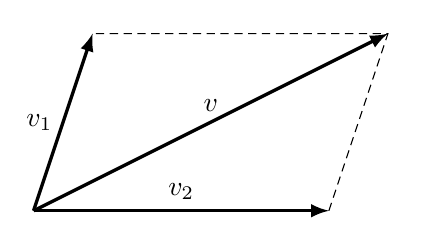
\begin{tikzpicture}[>=latex,scale=1.5]
  \useasboundingbox(-0.05,-0.05)rectangle(3.05,1.55);
  \draw [densely dashed](2.5,0)--(3,1.5) --(.5,1.5) ;
  \draw[->, very thick] (0,0)--node [above]{$v$}(3,1.5);
  \draw [->, very thick](0,0)--node [above]{$v_2$}(2.5,0);
  \draw [->, very thick](0,0)--node [left]{$v_1$}(.5,1.5);
\end{tikzpicture}
\end{document}